\documentclass{book}
\usepackage[a4paper,top=2.5cm,bottom=2.5cm,left=2.5cm,right=2.5cm]{geometry}
\usepackage{makeidx}
\usepackage{natbib}
\usepackage{graphicx}
\usepackage{multicol}
\usepackage{float}
\usepackage{listings}
\usepackage{color}
\usepackage{ifthen}
\usepackage[table]{xcolor}
\usepackage{textcomp}
\usepackage{alltt}
\usepackage{ifpdf}
\ifpdf
\usepackage[pdftex,
            pagebackref=true,
            colorlinks=true,
            linkcolor=blue,
            unicode
           ]{hyperref}
\else
\usepackage[ps2pdf,
            pagebackref=true,
            colorlinks=true,
            linkcolor=blue,
            unicode
           ]{hyperref}
\usepackage{pspicture}
\fi
\usepackage[utf8]{inputenc}
\usepackage{mathptmx}
\usepackage[scaled=.90]{helvet}
\usepackage{courier}
\usepackage{sectsty}
\usepackage{amssymb}
\usepackage[titles]{tocloft}
\usepackage{doxygen}
\lstset{language=C++,inputencoding=utf8,basicstyle=\footnotesize,breaklines=true,breakatwhitespace=true,tabsize=4,numbers=left }
\makeindex
\setcounter{tocdepth}{3}
\renewcommand{\footrulewidth}{0.4pt}
\renewcommand{\familydefault}{\sfdefault}
\hfuzz=15pt
\setlength{\emergencystretch}{15pt}
\hbadness=750
\tolerance=750
\begin{document}
\hypersetup{pageanchor=false,citecolor=blue}
\begin{titlepage}
\vspace*{7cm}
\begin{center}
{\Large libdxf\-\_\-2\-D \\[1ex]\large 0.\-1 }\\
\vspace*{1cm}
{\large Generated by Doxygen 1.8.3.1}\\
\vspace*{0.5cm}
{\small Mon Apr 29 2013 11:17:08}\\
\end{center}
\end{titlepage}
\clearemptydoublepage
\pagenumbering{roman}
\tableofcontents
\clearemptydoublepage
\pagenumbering{arabic}
\hypersetup{pageanchor=true,citecolor=blue}
\chapter{Main Page}
\label{index}\hypertarget{index}{}libdxf\-\_\-2\-D.\-so Library in C++

libdxf\-\_\-2\-D.\-so is a dynamic shared library made in C++. This library is used to generate D\-X\-F file that can be opened in Libre\-C\-A\-D 1.\-0.\-2. It can generate D\-X\-F file using line, rectangle and circle entities. This library also provides hatching feature. You can fill either with solid fill or pattern fill.

\subparagraph*{}

\subsection*{R\-E\-Q\-U\-I\-R\-E\-M\-E\-N\-T\-S\-:}

1) G\-N\-U G++ Compiler

Run following command in terminal to install \begin{DoxyVerb}    $ sudo apt-get install g++
\end{DoxyVerb}


\subparagraph*{}

\subsection*{I\-N\-S\-T\-A\-L\-L\-A\-T\-I\-O\-N\-:}

1) Open the terminal and type \begin{DoxyVerb}    $ git clone git://github.com/Akaur/testing.git
\end{DoxyVerb}


2) Go to this directory \begin{DoxyVerb}    $ cd testing
\end{DoxyVerb}


3) Run make \begin{DoxyVerb}    $ make\end{DoxyVerb}
 
\chapter{Hierarchical Index}
\section{Class Hierarchy}
This inheritance list is sorted roughly, but not completely, alphabetically\-:\begin{DoxyCompactList}
\item \contentsline{section}{base}{\pageref{classbase}}{}
\begin{DoxyCompactList}
\item \contentsline{section}{circle}{\pageref{classcircle}}{}
\item \contentsline{section}{dxf}{\pageref{classdxf}}{}
\item \contentsline{section}{line}{\pageref{classline}}{}
\item \contentsline{section}{rectangle}{\pageref{classrectangle}}{}
\end{DoxyCompactList}
\item \contentsline{section}{point}{\pageref{classpoint}}{}
\end{DoxyCompactList}

\chapter{Class Index}
\section{Class List}
Here are the classes, structs, unions and interfaces with brief descriptions\-:\begin{DoxyCompactList}
\item\contentsline{section}{\hyperlink{classbase}{base} \\*Base class defines functions for D\-X\-F header, footer and hatching section }{\pageref{classbase}}{}
\item\contentsline{section}{\hyperlink{classcircle}{circle} \\*Circle entity class }{\pageref{classcircle}}{}
\item\contentsline{section}{\hyperlink{classdxf}{dxf} \\*Draw entities in D\-X\-F file }{\pageref{classdxf}}{}
\item\contentsline{section}{\hyperlink{classline}{line} \\*Line entity class }{\pageref{classline}}{}
\item\contentsline{section}{\hyperlink{classpoint}{point} \\*Point entity class }{\pageref{classpoint}}{}
\item\contentsline{section}{\hyperlink{classrectangle}{rectangle} \\*Rectangle entity class }{\pageref{classrectangle}}{}
\end{DoxyCompactList}

\chapter{File Index}
\section{File List}
Here is a list of all documented files with brief descriptions\-:\begin{DoxyCompactList}
\item\contentsline{section}{include/\hyperlink{dxf__2D_8h}{dxf\-\_\-2\-D.\-h} }{\pageref{dxf__2D_8h}}{}
\item\contentsline{section}{src/\hyperlink{dxf__base_8cpp}{dxf\-\_\-base.\-cpp} \\*This file defines base class. base class is used to write header, footer and common hatching part to D\-X\-F file }{\pageref{dxf__base_8cpp}}{}
\item\contentsline{section}{src/\hyperlink{dxf__circle_8cpp}{dxf\-\_\-circle.\-cpp} \\*This file defines circle class. circle class is used to create circle entity with or without hatching }{\pageref{dxf__circle_8cpp}}{}
\item\contentsline{section}{src/\hyperlink{dxf__dxf_8cpp}{dxf\-\_\-dxf.\-cpp} \\*This file defines dxf class. dxf class is used to draw multiple entites in a D\-X\-F file }{\pageref{dxf__dxf_8cpp}}{}
\item\contentsline{section}{src/\hyperlink{dxf__line_8cpp}{dxf\-\_\-line.\-cpp} \\*This file is defining line class. line class is used to create line entity }{\pageref{dxf__line_8cpp}}{}
\item\contentsline{section}{src/\hyperlink{dxf__point_8cpp}{dxf\-\_\-point.\-cpp} \\*This file defines point class. point class is used to initialize x\-Co, y\-Co and z\-Co coordinates of point }{\pageref{dxf__point_8cpp}}{}
\item\contentsline{section}{src/\hyperlink{dxf__rect_8cpp}{dxf\-\_\-rect.\-cpp} \\*This file defines rectangle class. rectangle class is used to create rectangle with or without hatching }{\pageref{dxf__rect_8cpp}}{}
\item\contentsline{section}{test/{\bfseries example.\-cpp} }{\pageref{example_8cpp}}{}
\end{DoxyCompactList}

\chapter{Class Documentation}
\hypertarget{classbase}{\section{base Class Reference}
\label{classbase}\index{base@{base}}
}


Base class defines functions for D\-X\-F header, footer and hatching section.  




{\ttfamily \#include $<$dxf\-\_\-2\-D.\-h$>$}

Inheritance diagram for base\-:\begin{figure}[H]
\begin{center}
\leavevmode
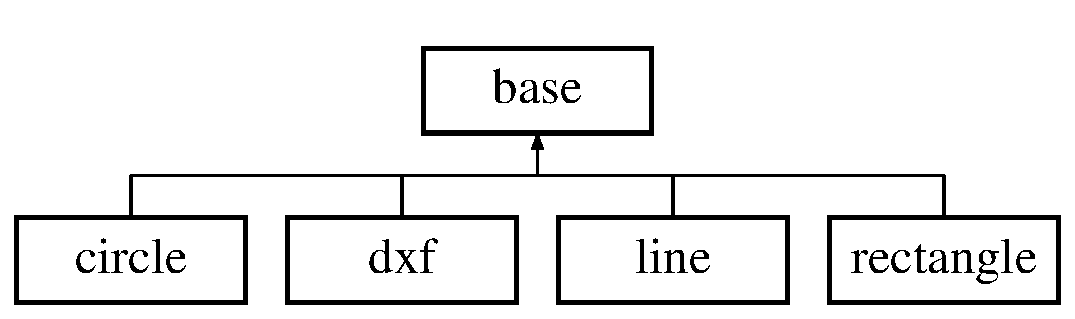
\includegraphics[height=2.000000cm]{classbase}
\end{center}
\end{figure}
\subsection*{Public Member Functions}
\begin{DoxyCompactItemize}
\item 
void \hyperlink{classbase_a7db4428cce94f69118405d98e6c239ee}{read\-\_\-\-Header} ()
\begin{DoxyCompactList}\small\item\em Reads D\-X\-F header. \end{DoxyCompactList}\item 
void \hyperlink{classbase_a03a4fcadee3375d5cb13195f82784450}{read\-\_\-\-Footer} ()
\begin{DoxyCompactList}\small\item\em Reads D\-X\-F E\-O\-F section. \end{DoxyCompactList}\item 
void \hyperlink{classbase_af4743cfcd16393cfc86bbcfd854a0727}{write\-\_\-\-Hatch\-\_\-\-Start} (int, string, int)
\begin{DoxyCompactList}\small\item\em Writes Hatch entity start part. \end{DoxyCompactList}\item 
void \hyperlink{classbase_acae9199dd5ca813b319665e8aa963bad}{write\-\_\-\-Hatch\-\_\-\-End} ()
\begin{DoxyCompactList}\small\item\em Writes hatch entity end part. \end{DoxyCompactList}\end{DoxyCompactItemize}
\subsection*{Public Attributes}
\begin{DoxyCompactItemize}
\item 
ofstream \hyperlink{classbase_a1a4cdb81a9c9f77818a0fdd34165a1ab}{write\-File}
\end{DoxyCompactItemize}
\subsection*{Protected Attributes}
\begin{DoxyCompactItemize}
\item 
double \hyperlink{classbase_a7703056e2be3f7e97f974e77146c3a02}{x\-Start}
\item 
double \hyperlink{classbase_a11d50718a751a277f133430692b13bbf}{y\-Start}
\item 
double \hyperlink{classbase_aa53533269b638644cb48a1cafc969852}{z\-Start}
\item 
double \hyperlink{classbase_aa4702751e837e49dcb88eaf2944f3c1f}{x\-End}
\item 
double \hyperlink{classbase_aa5a4fed2eaf64367a8ef693d8d054081}{y\-End}
\item 
double \hyperlink{classbase_ad599903bf17e619b3fe11c592f981682}{z\-End}
\item 
double \hyperlink{classbase_a83f02880ca88c37fcb28acced4d6b9a7}{x\-Mid}
\item 
double \hyperlink{classbase_acb79a7b7e25b442e350a151626f8aa46}{y\-Mid}
\item 
double \hyperlink{classbase_a36bed779447a9b6e7a902dc1d065ffb2}{radius}
\item 
ifstream \hyperlink{classbase_a707f4830c851eb50e9e2299fae731075}{read\-File}
\item 
int \hyperlink{classbase_ac16efe03b1a537989afd2a1eebdde0e9}{flag}
\item 
int \hyperlink{classbase_af5da8689af8a9b1bf5376873bbece1ae}{edges}
\item 
int \hyperlink{classbase_a65b11e6006cd45d381b31d6fbaa82c67}{edge\-\_\-type}
\item 
int \hyperlink{classbase_af8027c0e104b55838579c8cae311b558}{color}
\item 
string \hyperlink{classbase_aa3e204024e466de567044e1e992d39db}{dxf\-\_\-filename}
\item 
string \hyperlink{classbase_a8d165e9a0576b127d61404745e4deb1a}{readwrite}
\item 
string \hyperlink{classbase_a7ea31106027652ddba7c37809cade6ac}{pattern\-\_\-name}
\item 
string \hyperlink{classbase_adc118bdac066f100bb2ce0fa6d1cd657}{name}
\item 
string \hyperlink{classbase_ace32e46b9aa7521f7523e57e148dd248}{layer}
\end{DoxyCompactItemize}


\subsection{Detailed Description}
Base class defines functions for D\-X\-F header, footer and hatching section. 

Definition at line 35 of file dxf\-\_\-2\-D.\-h.



\subsection{Member Function Documentation}
\hypertarget{classbase_a03a4fcadee3375d5cb13195f82784450}{\index{base@{base}!read\-\_\-\-Footer@{read\-\_\-\-Footer}}
\index{read\-\_\-\-Footer@{read\-\_\-\-Footer}!base@{base}}
\subsubsection[{read\-\_\-\-Footer}]{\setlength{\rightskip}{0pt plus 5cm}void base\-::read\-\_\-\-Footer (
\begin{DoxyParamCaption}
{}
\end{DoxyParamCaption}
)}}\label{classbase_a03a4fcadee3375d5cb13195f82784450}


Reads D\-X\-F E\-O\-F section. 

Opens \char`\"{}dxf\-\_\-footer.\-txt\char`\"{} for reading and writes at the end of output D\-X\-F file. 

Definition at line 56 of file dxf\-\_\-base.\-cpp.

\hypertarget{classbase_a7db4428cce94f69118405d98e6c239ee}{\index{base@{base}!read\-\_\-\-Header@{read\-\_\-\-Header}}
\index{read\-\_\-\-Header@{read\-\_\-\-Header}!base@{base}}
\subsubsection[{read\-\_\-\-Header}]{\setlength{\rightskip}{0pt plus 5cm}void base\-::read\-\_\-\-Header (
\begin{DoxyParamCaption}
{}
\end{DoxyParamCaption}
)}}\label{classbase_a7db4428cce94f69118405d98e6c239ee}


Reads D\-X\-F header. 

Opens \char`\"{}dxf\-\_\-header.\-txt\char`\"{} file for reading and writes at the start of D\-X\-F file. 

Definition at line 30 of file dxf\-\_\-base.\-cpp.

\hypertarget{classbase_acae9199dd5ca813b319665e8aa963bad}{\index{base@{base}!write\-\_\-\-Hatch\-\_\-\-End@{write\-\_\-\-Hatch\-\_\-\-End}}
\index{write\-\_\-\-Hatch\-\_\-\-End@{write\-\_\-\-Hatch\-\_\-\-End}!base@{base}}
\subsubsection[{write\-\_\-\-Hatch\-\_\-\-End}]{\setlength{\rightskip}{0pt plus 5cm}void base\-::write\-\_\-\-Hatch\-\_\-\-End (
\begin{DoxyParamCaption}
{}
\end{DoxyParamCaption}
)}}\label{classbase_acae9199dd5ca813b319665e8aa963bad}


Writes hatch entity end part. 

Writes the common end part of hatch entity to the entity section of output D\-X\-F file. 

Definition at line 106 of file dxf\-\_\-base.\-cpp.

\hypertarget{classbase_af4743cfcd16393cfc86bbcfd854a0727}{\index{base@{base}!write\-\_\-\-Hatch\-\_\-\-Start@{write\-\_\-\-Hatch\-\_\-\-Start}}
\index{write\-\_\-\-Hatch\-\_\-\-Start@{write\-\_\-\-Hatch\-\_\-\-Start}!base@{base}}
\subsubsection[{write\-\_\-\-Hatch\-\_\-\-Start}]{\setlength{\rightskip}{0pt plus 5cm}void base\-::write\-\_\-\-Hatch\-\_\-\-Start (
\begin{DoxyParamCaption}
\item[{int}]{flag, }
\item[{string}]{pattern\-\_\-name, }
\item[{int}]{color}
\end{DoxyParamCaption}
)}}\label{classbase_af4743cfcd16393cfc86bbcfd854a0727}


Writes Hatch entity start part. 

Writes the common start part of hatch entity to the the entity section of D\-X\-F output file. 

Definition at line 82 of file dxf\-\_\-base.\-cpp.



\subsection{Member Data Documentation}
\hypertarget{classbase_af8027c0e104b55838579c8cae311b558}{\index{base@{base}!color@{color}}
\index{color@{color}!base@{base}}
\subsubsection[{color}]{\setlength{\rightskip}{0pt plus 5cm}int base\-::color\hspace{0.3cm}{\ttfamily [protected]}}}\label{classbase_af8027c0e104b55838579c8cae311b558}
color-\/code\mbox{[}1-\/256\mbox{]} 

Definition at line 51 of file dxf\-\_\-2\-D.\-h.

\hypertarget{classbase_aa3e204024e466de567044e1e992d39db}{\index{base@{base}!dxf\-\_\-filename@{dxf\-\_\-filename}}
\index{dxf\-\_\-filename@{dxf\-\_\-filename}!base@{base}}
\subsubsection[{dxf\-\_\-filename}]{\setlength{\rightskip}{0pt plus 5cm}string base\-::dxf\-\_\-filename\hspace{0.3cm}{\ttfamily [protected]}}}\label{classbase_aa3e204024e466de567044e1e992d39db}
output dxf filename 

Definition at line 57 of file dxf\-\_\-2\-D.\-h.

\hypertarget{classbase_a65b11e6006cd45d381b31d6fbaa82c67}{\index{base@{base}!edge\-\_\-type@{edge\-\_\-type}}
\index{edge\-\_\-type@{edge\-\_\-type}!base@{base}}
\subsubsection[{edge\-\_\-type}]{\setlength{\rightskip}{0pt plus 5cm}int base\-::edge\-\_\-type\hspace{0.3cm}{\ttfamily [protected]}}}\label{classbase_a65b11e6006cd45d381b31d6fbaa82c67}
boundary edge type 

Definition at line 51 of file dxf\-\_\-2\-D.\-h.

\hypertarget{classbase_af5da8689af8a9b1bf5376873bbece1ae}{\index{base@{base}!edges@{edges}}
\index{edges@{edges}!base@{base}}
\subsubsection[{edges}]{\setlength{\rightskip}{0pt plus 5cm}int base\-::edges\hspace{0.3cm}{\ttfamily [protected]}}}\label{classbase_af5da8689af8a9b1bf5376873bbece1ae}
edges of boundary path 

Definition at line 51 of file dxf\-\_\-2\-D.\-h.

\hypertarget{classbase_ac16efe03b1a537989afd2a1eebdde0e9}{\index{base@{base}!flag@{flag}}
\index{flag@{flag}!base@{base}}
\subsubsection[{flag}]{\setlength{\rightskip}{0pt plus 5cm}int base\-::flag\hspace{0.3cm}{\ttfamily [protected]}}}\label{classbase_ac16efe03b1a537989afd2a1eebdde0e9}
flag for hatching 

Definition at line 51 of file dxf\-\_\-2\-D.\-h.

\hypertarget{classbase_ace32e46b9aa7521f7523e57e148dd248}{\index{base@{base}!layer@{layer}}
\index{layer@{layer}!base@{base}}
\subsubsection[{layer}]{\setlength{\rightskip}{0pt plus 5cm}string base\-::layer\hspace{0.3cm}{\ttfamily [protected]}}}\label{classbase_ace32e46b9aa7521f7523e57e148dd248}
layer\mbox{[}0-\/5\mbox{]} 

Definition at line 57 of file dxf\-\_\-2\-D.\-h.

\hypertarget{classbase_adc118bdac066f100bb2ce0fa6d1cd657}{\index{base@{base}!name@{name}}
\index{name@{name}!base@{base}}
\subsubsection[{name}]{\setlength{\rightskip}{0pt plus 5cm}string base\-::name\hspace{0.3cm}{\ttfamily [protected]}}}\label{classbase_adc118bdac066f100bb2ce0fa6d1cd657}
input filename for reading 

Definition at line 57 of file dxf\-\_\-2\-D.\-h.

\hypertarget{classbase_a7ea31106027652ddba7c37809cade6ac}{\index{base@{base}!pattern\-\_\-name@{pattern\-\_\-name}}
\index{pattern\-\_\-name@{pattern\-\_\-name}!base@{base}}
\subsubsection[{pattern\-\_\-name}]{\setlength{\rightskip}{0pt plus 5cm}string base\-::pattern\-\_\-name\hspace{0.3cm}{\ttfamily [protected]}}}\label{classbase_a7ea31106027652ddba7c37809cade6ac}
pattern name for pattern hatching 

Definition at line 57 of file dxf\-\_\-2\-D.\-h.

\hypertarget{classbase_a36bed779447a9b6e7a902dc1d065ffb2}{\index{base@{base}!radius@{radius}}
\index{radius@{radius}!base@{base}}
\subsubsection[{radius}]{\setlength{\rightskip}{0pt plus 5cm}double base\-::radius\hspace{0.3cm}{\ttfamily [protected]}}}\label{classbase_a36bed779447a9b6e7a902dc1d065ffb2}
radius of circle 

Definition at line 39 of file dxf\-\_\-2\-D.\-h.

\hypertarget{classbase_a707f4830c851eb50e9e2299fae731075}{\index{base@{base}!read\-File@{read\-File}}
\index{read\-File@{read\-File}!base@{base}}
\subsubsection[{read\-File}]{\setlength{\rightskip}{0pt plus 5cm}ifstream base\-::read\-File\hspace{0.3cm}{\ttfamily [protected]}}}\label{classbase_a707f4830c851eb50e9e2299fae731075}
object for reading files 

Definition at line 49 of file dxf\-\_\-2\-D.\-h.

\hypertarget{classbase_a8d165e9a0576b127d61404745e4deb1a}{\index{base@{base}!readwrite@{readwrite}}
\index{readwrite@{readwrite}!base@{base}}
\subsubsection[{readwrite}]{\setlength{\rightskip}{0pt plus 5cm}string base\-::readwrite\hspace{0.3cm}{\ttfamily [protected]}}}\label{classbase_a8d165e9a0576b127d61404745e4deb1a}
reads from input file and writes to output file 

Definition at line 57 of file dxf\-\_\-2\-D.\-h.

\hypertarget{classbase_a1a4cdb81a9c9f77818a0fdd34165a1ab}{\index{base@{base}!write\-File@{write\-File}}
\index{write\-File@{write\-File}!base@{base}}
\subsubsection[{write\-File}]{\setlength{\rightskip}{0pt plus 5cm}ofstream base\-::write\-File}}\label{classbase_a1a4cdb81a9c9f77818a0fdd34165a1ab}
object for writing files 

Definition at line 66 of file dxf\-\_\-2\-D.\-h.

\hypertarget{classbase_aa4702751e837e49dcb88eaf2944f3c1f}{\index{base@{base}!x\-End@{x\-End}}
\index{x\-End@{x\-End}!base@{base}}
\subsubsection[{x\-End}]{\setlength{\rightskip}{0pt plus 5cm}double base\-::x\-End\hspace{0.3cm}{\ttfamily [protected]}}}\label{classbase_aa4702751e837e49dcb88eaf2944f3c1f}
x-\/coordinate of ending point(x2, y2, z2) 

Definition at line 39 of file dxf\-\_\-2\-D.\-h.

\hypertarget{classbase_a83f02880ca88c37fcb28acced4d6b9a7}{\index{base@{base}!x\-Mid@{x\-Mid}}
\index{x\-Mid@{x\-Mid}!base@{base}}
\subsubsection[{x\-Mid}]{\setlength{\rightskip}{0pt plus 5cm}double base\-::x\-Mid\hspace{0.3cm}{\ttfamily [protected]}}}\label{classbase_a83f02880ca88c37fcb28acced4d6b9a7}
x-\/coordinate of center(x, y) for circle 

Definition at line 39 of file dxf\-\_\-2\-D.\-h.

\hypertarget{classbase_a7703056e2be3f7e97f974e77146c3a02}{\index{base@{base}!x\-Start@{x\-Start}}
\index{x\-Start@{x\-Start}!base@{base}}
\subsubsection[{x\-Start}]{\setlength{\rightskip}{0pt plus 5cm}double base\-::x\-Start\hspace{0.3cm}{\ttfamily [protected]}}}\label{classbase_a7703056e2be3f7e97f974e77146c3a02}
x-\/coordinate of starting point(x1, y1, z1) 

Definition at line 39 of file dxf\-\_\-2\-D.\-h.

\hypertarget{classbase_aa5a4fed2eaf64367a8ef693d8d054081}{\index{base@{base}!y\-End@{y\-End}}
\index{y\-End@{y\-End}!base@{base}}
\subsubsection[{y\-End}]{\setlength{\rightskip}{0pt plus 5cm}double base\-::y\-End\hspace{0.3cm}{\ttfamily [protected]}}}\label{classbase_aa5a4fed2eaf64367a8ef693d8d054081}
y-\/coordinate of ending point(x2, y2, z2) 

Definition at line 39 of file dxf\-\_\-2\-D.\-h.

\hypertarget{classbase_acb79a7b7e25b442e350a151626f8aa46}{\index{base@{base}!y\-Mid@{y\-Mid}}
\index{y\-Mid@{y\-Mid}!base@{base}}
\subsubsection[{y\-Mid}]{\setlength{\rightskip}{0pt plus 5cm}double base\-::y\-Mid\hspace{0.3cm}{\ttfamily [protected]}}}\label{classbase_acb79a7b7e25b442e350a151626f8aa46}
y-\/coordinate of center(x, y) for circle 

Definition at line 39 of file dxf\-\_\-2\-D.\-h.

\hypertarget{classbase_a11d50718a751a277f133430692b13bbf}{\index{base@{base}!y\-Start@{y\-Start}}
\index{y\-Start@{y\-Start}!base@{base}}
\subsubsection[{y\-Start}]{\setlength{\rightskip}{0pt plus 5cm}double base\-::y\-Start\hspace{0.3cm}{\ttfamily [protected]}}}\label{classbase_a11d50718a751a277f133430692b13bbf}
y-\/coordinate of starting point(x1, y1, z1) 

Definition at line 39 of file dxf\-\_\-2\-D.\-h.

\hypertarget{classbase_ad599903bf17e619b3fe11c592f981682}{\index{base@{base}!z\-End@{z\-End}}
\index{z\-End@{z\-End}!base@{base}}
\subsubsection[{z\-End}]{\setlength{\rightskip}{0pt plus 5cm}double base\-::z\-End\hspace{0.3cm}{\ttfamily [protected]}}}\label{classbase_ad599903bf17e619b3fe11c592f981682}
z-\/coordinate of ending point(x2, y2, z2) 

Definition at line 39 of file dxf\-\_\-2\-D.\-h.

\hypertarget{classbase_aa53533269b638644cb48a1cafc969852}{\index{base@{base}!z\-Start@{z\-Start}}
\index{z\-Start@{z\-Start}!base@{base}}
\subsubsection[{z\-Start}]{\setlength{\rightskip}{0pt plus 5cm}double base\-::z\-Start\hspace{0.3cm}{\ttfamily [protected]}}}\label{classbase_aa53533269b638644cb48a1cafc969852}
z-\/coordinate of starting point(x1, y1, z1) 

Definition at line 39 of file dxf\-\_\-2\-D.\-h.



The documentation for this class was generated from the following files\-:\begin{DoxyCompactItemize}
\item 
include/\hyperlink{dxf__2D_8h}{dxf\-\_\-2\-D.\-h}\item 
src/\hyperlink{dxf__base_8cpp}{dxf\-\_\-base.\-cpp}\end{DoxyCompactItemize}

\hypertarget{classcircle}{\section{circle Class Reference}
\label{classcircle}\index{circle@{circle}}
}


Circle entity class.  




{\ttfamily \#include $<$dxf\-\_\-2\-D.\-h$>$}

Inheritance diagram for circle\-:\begin{figure}[H]
\begin{center}
\leavevmode
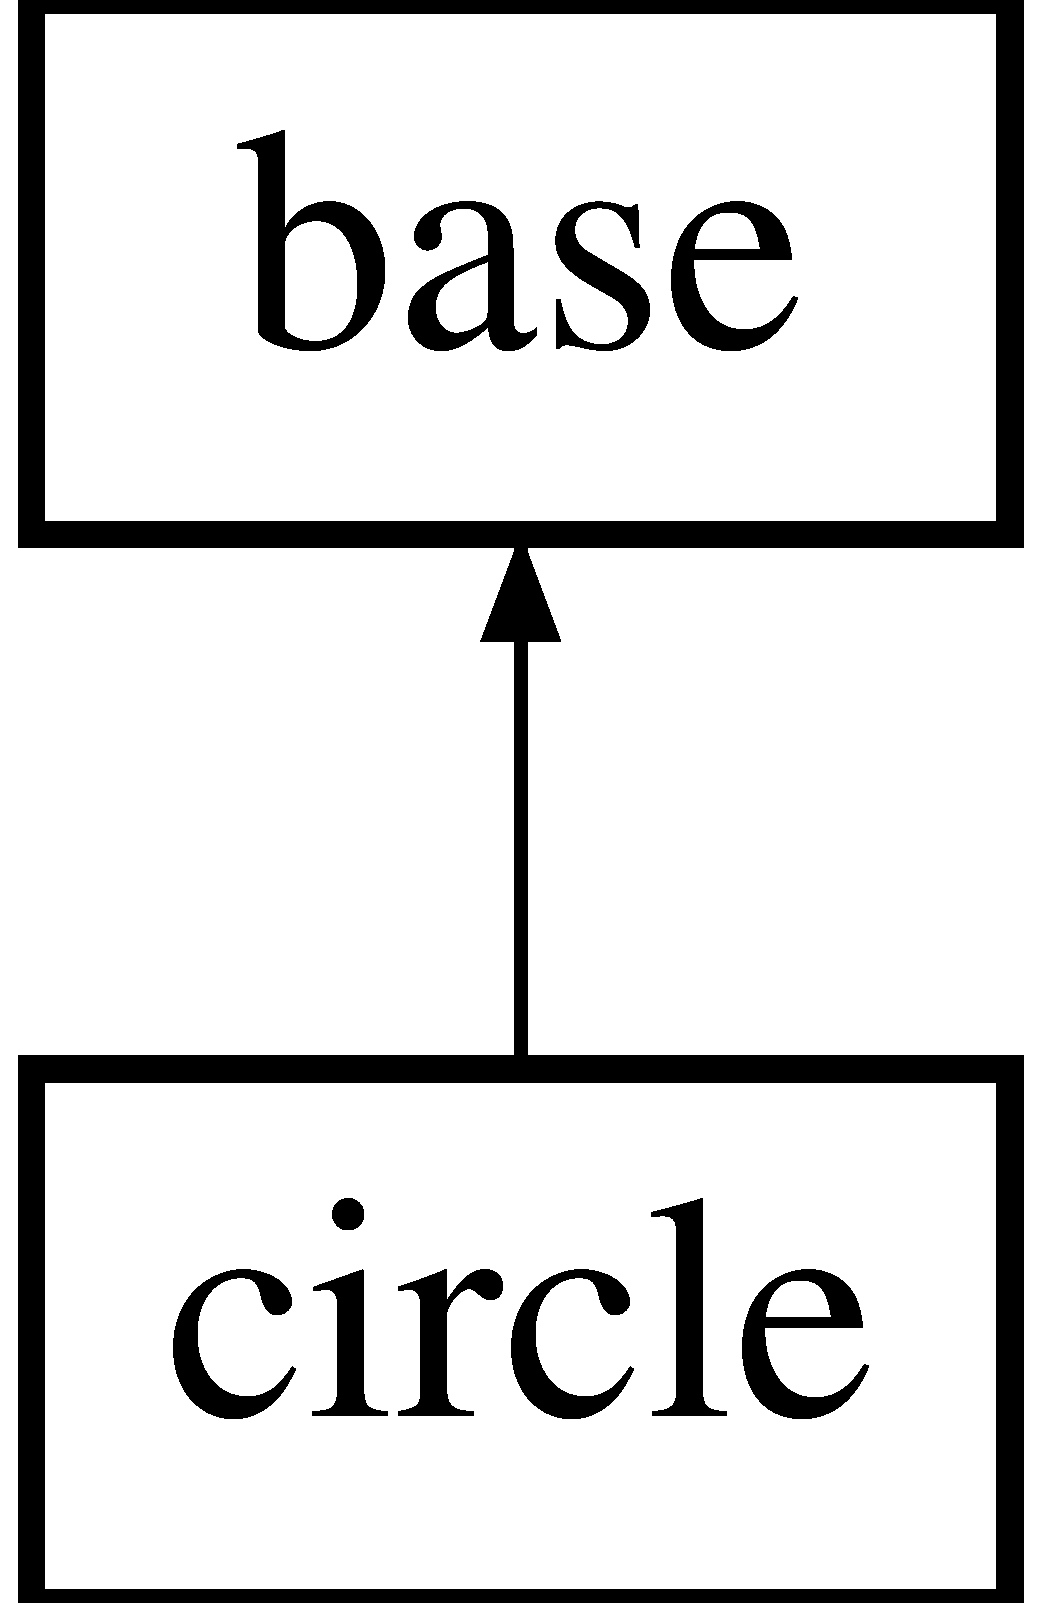
\includegraphics[height=2.000000cm]{classcircle}
\end{center}
\end{figure}
\subsection*{Public Member Functions}
\begin{DoxyCompactItemize}
\item 
\hypertarget{classcircle_a4e0786fc75051f3bbe5de2e08ef9712d}{\hyperlink{classcircle_a4e0786fc75051f3bbe5de2e08ef9712d}{circle} ()}\label{classcircle_a4e0786fc75051f3bbe5de2e08ef9712d}

\begin{DoxyCompactList}\small\item\em Default constructor. \end{DoxyCompactList}\item 
\hyperlink{classcircle_a265f35d522e8d1bf2a3953146caec09e}{circle} (\hyperlink{classpoint}{point} \&, double, string, \hyperlink{classdxf}{dxf} \&)
\begin{DoxyCompactList}\small\item\em Parameterized constructor. \end{DoxyCompactList}\item 
\hyperlink{classcircle_a6824eba724e2ec93029fd50423d13008}{circle} (\hyperlink{classpoint}{point} \&, double, string, \hyperlink{classdxf}{dxf} \&, int hflag, int hcolor=256)
\begin{DoxyCompactList}\small\item\em Parameterized constructor for solid fill. \end{DoxyCompactList}\item 
\hyperlink{classcircle_a4a17fabc4fe9f4da10f30cd8272ed8b5}{circle} (\hyperlink{classpoint}{point} \&, double, string, \hyperlink{classdxf}{dxf} \&, int hflag, string p\-\_\-name, int hcolor=256)
\begin{DoxyCompactList}\small\item\em Parameterized constructor for pattern fill. \end{DoxyCompactList}\end{DoxyCompactItemize}
\subsection*{Additional Inherited Members}


\subsection{Detailed Description}
Circle entity class. 

Definition at line 192 of file dxf\-\_\-2\-D.\-h.



\subsection{Constructor \& Destructor Documentation}
\hypertarget{classcircle_a265f35d522e8d1bf2a3953146caec09e}{\index{circle@{circle}!circle@{circle}}
\index{circle@{circle}!circle@{circle}}
\subsubsection[{circle}]{\setlength{\rightskip}{0pt plus 5cm}circle\-::circle (
\begin{DoxyParamCaption}
\item[{{\bf point} \&}]{pt1, }
\item[{double}]{r, }
\item[{string}]{dlayer, }
\item[{{\bf dxf} \&}]{d}
\end{DoxyParamCaption}
)}}\label{classcircle_a265f35d522e8d1bf2a3953146caec09e}


Parameterized constructor. 

Initializes starting point and radius of circle, specify the layer and calls write\-\_\-\-Circle(x\-Start, y\-Start, z\-Start, radius, layer) function of dxf class for writing circle. entity to D\-X\-F file. 

Definition at line 45 of file dxf\-\_\-circle.\-cpp.

\hypertarget{classcircle_a6824eba724e2ec93029fd50423d13008}{\index{circle@{circle}!circle@{circle}}
\index{circle@{circle}!circle@{circle}}
\subsubsection[{circle}]{\setlength{\rightskip}{0pt plus 5cm}circle\-::circle (
\begin{DoxyParamCaption}
\item[{{\bf point} \&}]{pt1, }
\item[{double}]{r, }
\item[{string}]{dlayer, }
\item[{{\bf dxf} \&}]{d, }
\item[{int}]{hflag, }
\item[{int}]{hcolor = {\ttfamily 256}}
\end{DoxyParamCaption}
)}}\label{classcircle_a6824eba724e2ec93029fd50423d13008}


Parameterized constructor for solid fill. 

Initialize starting point and radius of circle, specify the layer, flag = 1 for solid fill and calls write\-\_\-\-Circle(x\-Start, y\-Start, z\-Start, radius, layer, flag, color) function of dxf class for writing circle (solid fill) entity to D\-X\-F file. 

Definition at line 74 of file dxf\-\_\-circle.\-cpp.

\hypertarget{classcircle_a4a17fabc4fe9f4da10f30cd8272ed8b5}{\index{circle@{circle}!circle@{circle}}
\index{circle@{circle}!circle@{circle}}
\subsubsection[{circle}]{\setlength{\rightskip}{0pt plus 5cm}circle\-::circle (
\begin{DoxyParamCaption}
\item[{{\bf point} \&}]{pt1, }
\item[{double}]{r, }
\item[{string}]{dlayer, }
\item[{{\bf dxf} \&}]{d, }
\item[{int}]{hflag, }
\item[{string}]{p\-\_\-name, }
\item[{int}]{hcolor = {\ttfamily 256}}
\end{DoxyParamCaption}
)}}\label{classcircle_a4a17fabc4fe9f4da10f30cd8272ed8b5}


Parameterized constructor for pattern fill. 

Initialize starting point and radius of circle, specify the layer, flag = 0 for pattern fill and calls write\-\_\-\-Circle(x\-Start, y\-Start, z\-Start, radius, layer, flag, pattern\-\_\-name, color) function of dxf class for writing circle (pattern fill) entity to D\-X\-F file. 

Definition at line 107 of file dxf\-\_\-circle.\-cpp.



The documentation for this class was generated from the following files\-:\begin{DoxyCompactItemize}
\item 
include/\hyperlink{dxf__2D_8h}{dxf\-\_\-2\-D.\-h}\item 
src/\hyperlink{dxf__circle_8cpp}{dxf\-\_\-circle.\-cpp}\end{DoxyCompactItemize}

\hypertarget{classdxf}{\section{dxf Class Reference}
\label{classdxf}\index{dxf@{dxf}}
}


Draw entities in D\-X\-F file.  




{\ttfamily \#include $<$dxf\-\_\-2\-D.\-h$>$}

Inheritance diagram for dxf\-:\begin{figure}[H]
\begin{center}
\leavevmode
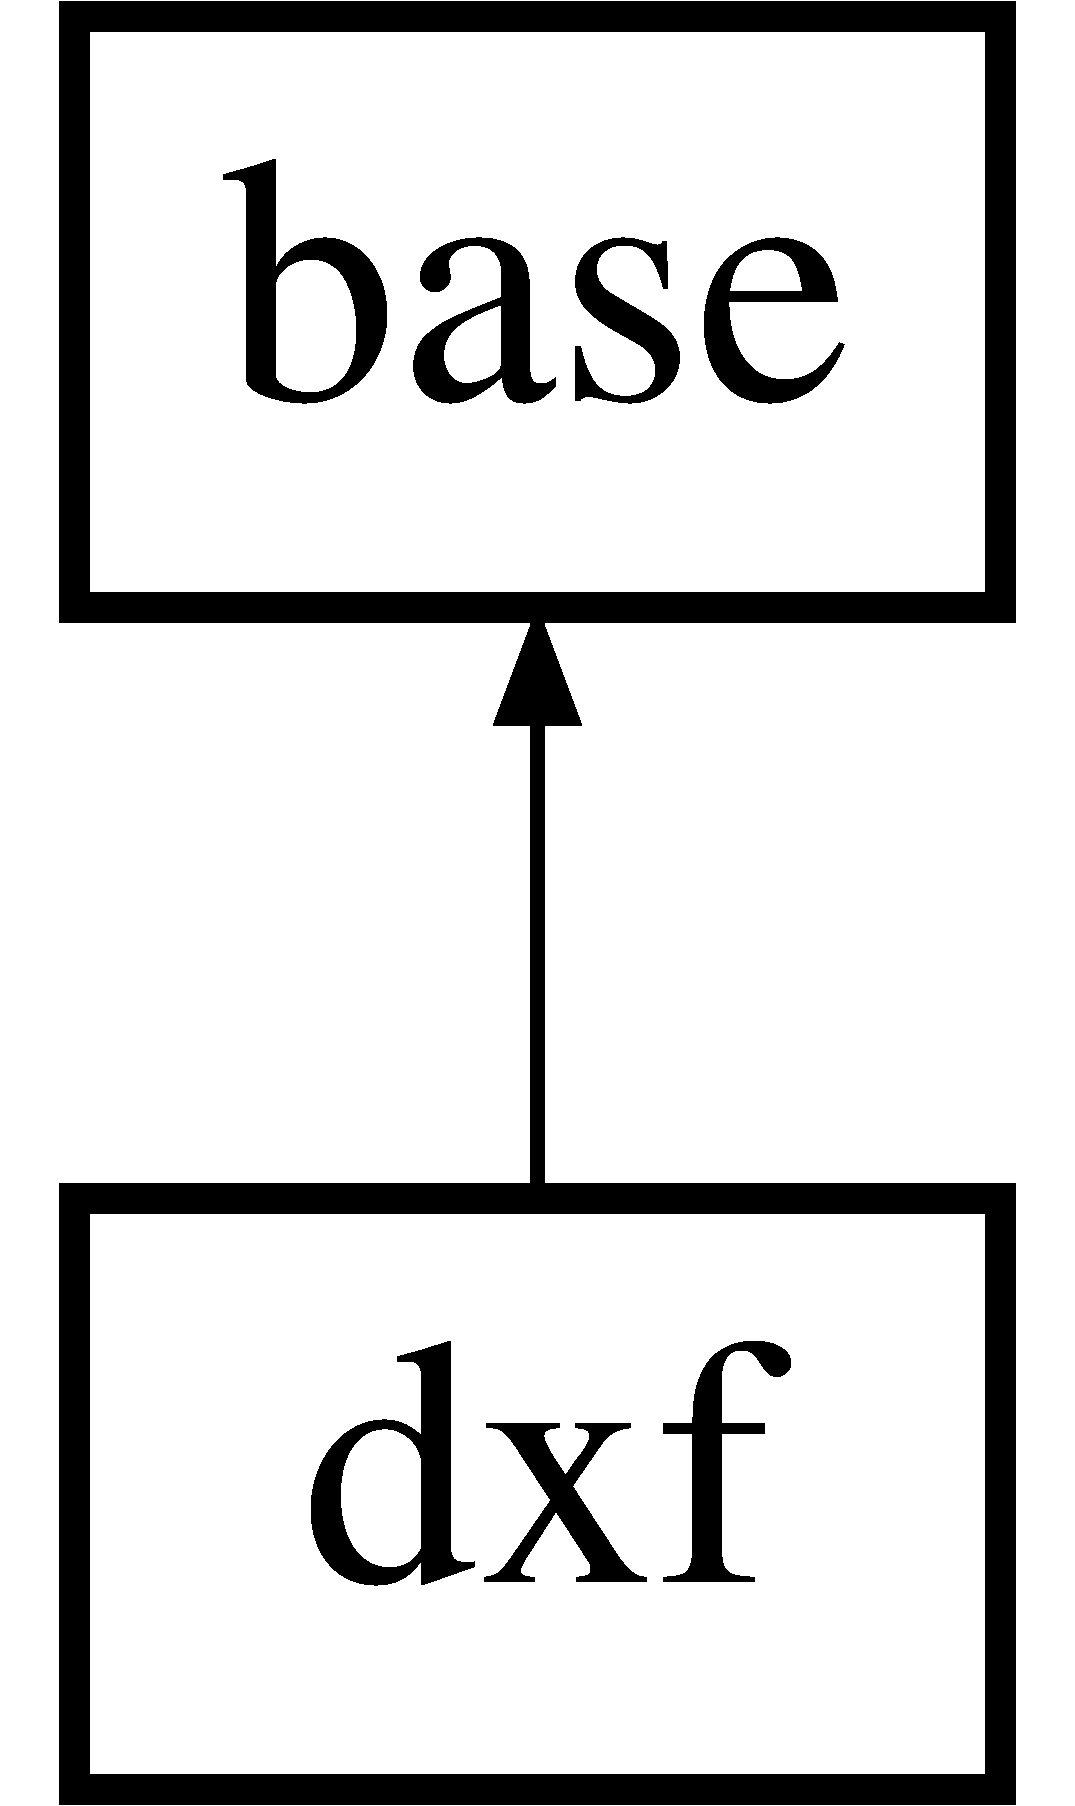
\includegraphics[height=2.000000cm]{classdxf}
\end{center}
\end{figure}
\subsection*{Public Member Functions}
\begin{DoxyCompactItemize}
\item 
\hypertarget{classdxf_ac4deaef37b2db70a0361104c66e0b481}{\hyperlink{classdxf_ac4deaef37b2db70a0361104c66e0b481}{dxf} ()}\label{classdxf_ac4deaef37b2db70a0361104c66e0b481}

\begin{DoxyCompactList}\small\item\em Default constructor. \end{DoxyCompactList}\item 
\hyperlink{classdxf_abae446dc642503b58fd45bcd22e08d78}{dxf} (string)
\begin{DoxyCompactList}\small\item\em Parameterised constructor. \end{DoxyCompactList}\item 
void \hyperlink{classdxf_a4daa6ebaa33481a5893d31095753fb09}{save} ()
\begin{DoxyCompactList}\small\item\em Save D\-X\-F file. \end{DoxyCompactList}\item 
void \hyperlink{classdxf_aa79b15af723a7df01acf575957e2104d}{write\-\_\-\-Line} (double, double, double, double, double, double, string)
\begin{DoxyCompactList}\small\item\em Line entity. \end{DoxyCompactList}\item 
void \hyperlink{classdxf_a45735534e1e6417003633a8a33ccebde}{write\-\_\-\-Circle} (double, double, double, double, string)
\begin{DoxyCompactList}\small\item\em Circle entity. \end{DoxyCompactList}\item 
void \hyperlink{classdxf_a62a9d48800f66a6811822264426a8ee0}{write\-\_\-\-Circle} (double, double, double, double, string, int, int)
\begin{DoxyCompactList}\small\item\em Circle (solid fill) entity. \end{DoxyCompactList}\item 
void \hyperlink{classdxf_a793fdaf19224abd12a239bcad0eda01b}{write\-\_\-\-Circle} (double, double, double, double, string, int, string, int)
\begin{DoxyCompactList}\small\item\em Circle (pattern fill) entity. \end{DoxyCompactList}\item 
void \hyperlink{classdxf_abc4eaf8ed68b05f25af6d31bd75ec3ce}{write\-\_\-\-Hatch\-\_\-\-Circle} (double, double, double, double)
\begin{DoxyCompactList}\small\item\em Hatch circle entity. \end{DoxyCompactList}\item 
void \hyperlink{classdxf_ae214af172af9ba53e10664cae1a53318}{write\-\_\-\-Rect} (double, double, double, double, double, double, string)
\begin{DoxyCompactList}\small\item\em Rectangle entity. \end{DoxyCompactList}\item 
void \hyperlink{classdxf_a67d61f8f015b73d585a5546ab915481d}{write\-\_\-\-Rect} (double, double, double, double, double, double, string, int, int)
\begin{DoxyCompactList}\small\item\em Rectangle (solid fill) entity. \end{DoxyCompactList}\item 
void \hyperlink{classdxf_ae6b53acc7a648fc435b25a8490947119}{write\-\_\-\-Rect} (double, double, double, double, double, double, string, int, string, int)
\begin{DoxyCompactList}\small\item\em Rectangle (pattern fill) entity. \end{DoxyCompactList}\item 
void \hyperlink{classdxf_ab4c7275d37a1151c9f2004d3711d5441}{write\-\_\-\-Hatch\-\_\-\-Rect} (double, double, double, double, double, double)
\begin{DoxyCompactList}\small\item\em Hatch rectangle entity. \end{DoxyCompactList}\end{DoxyCompactItemize}
\subsection*{Additional Inherited Members}


\subsection{Detailed Description}
Draw entities in D\-X\-F file. 

Definition at line 114 of file dxf\-\_\-2\-D.\-h.



\subsection{Constructor \& Destructor Documentation}
\hypertarget{classdxf_abae446dc642503b58fd45bcd22e08d78}{\index{dxf@{dxf}!dxf@{dxf}}
\index{dxf@{dxf}!dxf@{dxf}}
\subsubsection[{dxf}]{\setlength{\rightskip}{0pt plus 5cm}dxf\-::dxf (
\begin{DoxyParamCaption}
\item[{string}]{filename}
\end{DoxyParamCaption}
)}}\label{classdxf_abae446dc642503b58fd45bcd22e08d78}


Parameterised constructor. 

Constructor opens the filename for writing and writes D\-X\-F header to it. 

Definition at line 43 of file dxf\-\_\-dxf.\-cpp.



\subsection{Member Function Documentation}
\hypertarget{classdxf_a4daa6ebaa33481a5893d31095753fb09}{\index{dxf@{dxf}!save@{save}}
\index{save@{save}!dxf@{dxf}}
\subsubsection[{save}]{\setlength{\rightskip}{0pt plus 5cm}void dxf\-::save (
\begin{DoxyParamCaption}
{}
\end{DoxyParamCaption}
)}}\label{classdxf_a4daa6ebaa33481a5893d31095753fb09}


Save D\-X\-F file. 

Constructor closes D\-X\-F file after writing D\-X\-F footer to it. 

Definition at line 60 of file dxf\-\_\-dxf.\-cpp.

\hypertarget{classdxf_a45735534e1e6417003633a8a33ccebde}{\index{dxf@{dxf}!write\-\_\-\-Circle@{write\-\_\-\-Circle}}
\index{write\-\_\-\-Circle@{write\-\_\-\-Circle}!dxf@{dxf}}
\subsubsection[{write\-\_\-\-Circle}]{\setlength{\rightskip}{0pt plus 5cm}void dxf\-::write\-\_\-\-Circle (
\begin{DoxyParamCaption}
\item[{double}]{x\-Start, }
\item[{double}]{y\-Start, }
\item[{double}]{z\-Start, }
\item[{double}]{radius, }
\item[{string}]{layer}
\end{DoxyParamCaption}
)}}\label{classdxf_a45735534e1e6417003633a8a33ccebde}


Circle entity. 

Writes circle entity to D\-X\-F file. 

Definition at line 109 of file dxf\-\_\-dxf.\-cpp.

\hypertarget{classdxf_a62a9d48800f66a6811822264426a8ee0}{\index{dxf@{dxf}!write\-\_\-\-Circle@{write\-\_\-\-Circle}}
\index{write\-\_\-\-Circle@{write\-\_\-\-Circle}!dxf@{dxf}}
\subsubsection[{write\-\_\-\-Circle}]{\setlength{\rightskip}{0pt plus 5cm}void dxf\-::write\-\_\-\-Circle (
\begin{DoxyParamCaption}
\item[{double}]{x\-Start, }
\item[{double}]{y\-Start, }
\item[{double}]{z\-Start, }
\item[{double}]{radius, }
\item[{string}]{layer, }
\item[{int}]{flag, }
\item[{int}]{color}
\end{DoxyParamCaption}
)}}\label{classdxf_a62a9d48800f66a6811822264426a8ee0}


Circle (solid fill) entity. 

Writes circle (solid fill) entity to D\-X\-F file by calling write\-\_\-\-Hatch\-\_\-\-Start(flag, pattern\-\_\-name, color), write\-\_\-\-Hatch\-\_\-\-Circle(x\-Start, y\-Start, z\-Start, radius), \hyperlink{classbase_acae9199dd5ca813b319665e8aa963bad}{write\-\_\-\-Hatch\-\_\-\-End()} and write\-\_\-\-Circle(x\-Start, y\-Start, z\-Start, radius, layer). 

Definition at line 140 of file dxf\-\_\-dxf.\-cpp.

\hypertarget{classdxf_a793fdaf19224abd12a239bcad0eda01b}{\index{dxf@{dxf}!write\-\_\-\-Circle@{write\-\_\-\-Circle}}
\index{write\-\_\-\-Circle@{write\-\_\-\-Circle}!dxf@{dxf}}
\subsubsection[{write\-\_\-\-Circle}]{\setlength{\rightskip}{0pt plus 5cm}void dxf\-::write\-\_\-\-Circle (
\begin{DoxyParamCaption}
\item[{double}]{x\-Start, }
\item[{double}]{y\-Start, }
\item[{double}]{z\-Start, }
\item[{double}]{radius, }
\item[{string}]{layer, }
\item[{int}]{flag, }
\item[{string}]{pattern\-\_\-name, }
\item[{int}]{color}
\end{DoxyParamCaption}
)}}\label{classdxf_a793fdaf19224abd12a239bcad0eda01b}


Circle (pattern fill) entity. 

Writes circle (pattern fill) entity to D\-X\-F file by calling write\-\_\-\-Hatch\-\_\-\-Start(flag, pattern\-\_\-name, color), write\-\_\-\-Hatch\-\_\-\-Circle(x\-Start, y\-Start, z\-Start, radius), \hyperlink{classbase_acae9199dd5ca813b319665e8aa963bad}{write\-\_\-\-Hatch\-\_\-\-End()} and write\-\_\-\-Circle(x\-Start, y\-Start, z\-Start, radius, layer). 

Definition at line 169 of file dxf\-\_\-dxf.\-cpp.

\hypertarget{classdxf_abc4eaf8ed68b05f25af6d31bd75ec3ce}{\index{dxf@{dxf}!write\-\_\-\-Hatch\-\_\-\-Circle@{write\-\_\-\-Hatch\-\_\-\-Circle}}
\index{write\-\_\-\-Hatch\-\_\-\-Circle@{write\-\_\-\-Hatch\-\_\-\-Circle}!dxf@{dxf}}
\subsubsection[{write\-\_\-\-Hatch\-\_\-\-Circle}]{\setlength{\rightskip}{0pt plus 5cm}void dxf\-::write\-\_\-\-Hatch\-\_\-\-Circle (
\begin{DoxyParamCaption}
\item[{double}]{x\-Start, }
\item[{double}]{y\-Start, }
\item[{double}]{z\-Start, }
\item[{double}]{radius}
\end{DoxyParamCaption}
)}}\label{classdxf_abc4eaf8ed68b05f25af6d31bd75ec3ce}


Hatch circle entity. 

Writes hatch circle entity to D\-X\-F file. 

Definition at line 192 of file dxf\-\_\-dxf.\-cpp.

\hypertarget{classdxf_ab4c7275d37a1151c9f2004d3711d5441}{\index{dxf@{dxf}!write\-\_\-\-Hatch\-\_\-\-Rect@{write\-\_\-\-Hatch\-\_\-\-Rect}}
\index{write\-\_\-\-Hatch\-\_\-\-Rect@{write\-\_\-\-Hatch\-\_\-\-Rect}!dxf@{dxf}}
\subsubsection[{write\-\_\-\-Hatch\-\_\-\-Rect}]{\setlength{\rightskip}{0pt plus 5cm}void dxf\-::write\-\_\-\-Hatch\-\_\-\-Rect (
\begin{DoxyParamCaption}
\item[{double}]{x\-Start, }
\item[{double}]{y\-Start, }
\item[{double}]{z\-Start, }
\item[{double}]{x\-End, }
\item[{double}]{y\-End, }
\item[{double}]{z\-End}
\end{DoxyParamCaption}
)}}\label{classdxf_ab4c7275d37a1151c9f2004d3711d5441}


Hatch rectangle entity. 

Writes hatch rectangle entity to D\-X\-F file. 

Definition at line 303 of file dxf\-\_\-dxf.\-cpp.

\hypertarget{classdxf_aa79b15af723a7df01acf575957e2104d}{\index{dxf@{dxf}!write\-\_\-\-Line@{write\-\_\-\-Line}}
\index{write\-\_\-\-Line@{write\-\_\-\-Line}!dxf@{dxf}}
\subsubsection[{write\-\_\-\-Line}]{\setlength{\rightskip}{0pt plus 5cm}void dxf\-::write\-\_\-\-Line (
\begin{DoxyParamCaption}
\item[{double}]{x\-Start, }
\item[{double}]{y\-Start, }
\item[{double}]{z\-Start, }
\item[{double}]{x\-End, }
\item[{double}]{y\-End, }
\item[{double}]{z\-End, }
\item[{string}]{layer}
\end{DoxyParamCaption}
)}}\label{classdxf_aa79b15af723a7df01acf575957e2104d}


Line entity. 

Writes line entity to D\-X\-F file. 

Definition at line 78 of file dxf\-\_\-dxf.\-cpp.

\hypertarget{classdxf_ae214af172af9ba53e10664cae1a53318}{\index{dxf@{dxf}!write\-\_\-\-Rect@{write\-\_\-\-Rect}}
\index{write\-\_\-\-Rect@{write\-\_\-\-Rect}!dxf@{dxf}}
\subsubsection[{write\-\_\-\-Rect}]{\setlength{\rightskip}{0pt plus 5cm}void dxf\-::write\-\_\-\-Rect (
\begin{DoxyParamCaption}
\item[{double}]{x\-Start, }
\item[{double}]{y\-Start, }
\item[{double}]{z\-Start, }
\item[{double}]{x\-End, }
\item[{double}]{y\-End, }
\item[{double}]{z\-End, }
\item[{string}]{layer}
\end{DoxyParamCaption}
)}}\label{classdxf_ae214af172af9ba53e10664cae1a53318}


Rectangle entity. 

Writes rectangle entity to D\-X\-F file. 

Definition at line 213 of file dxf\-\_\-dxf.\-cpp.

\hypertarget{classdxf_a67d61f8f015b73d585a5546ab915481d}{\index{dxf@{dxf}!write\-\_\-\-Rect@{write\-\_\-\-Rect}}
\index{write\-\_\-\-Rect@{write\-\_\-\-Rect}!dxf@{dxf}}
\subsubsection[{write\-\_\-\-Rect}]{\setlength{\rightskip}{0pt plus 5cm}void dxf\-::write\-\_\-\-Rect (
\begin{DoxyParamCaption}
\item[{double}]{x\-Start, }
\item[{double}]{y\-Start, }
\item[{double}]{z\-Start, }
\item[{double}]{x\-End, }
\item[{double}]{y\-End, }
\item[{double}]{z\-End, }
\item[{string}]{layer, }
\item[{int}]{flag, }
\item[{int}]{color}
\end{DoxyParamCaption}
)}}\label{classdxf_a67d61f8f015b73d585a5546ab915481d}


Rectangle (solid fill) entity. 

Writes rectangle (solid fill) entity to D\-X\-F file by calling write\-\_\-\-Hatch\-\_\-\-Start(flag, pattern\-\_\-name, color), write\-\_\-\-Hatch\-\_\-\-Rect(x\-Start, y\-Start, z\-Start, x\-End, y\-End, z\-End), \hyperlink{classbase_acae9199dd5ca813b319665e8aa963bad}{write\-\_\-\-Hatch\-\_\-\-End()} and write\-\_\-\-Rect(x\-Start, y\-Start, z\-Start, x\-End, y\-End, z\-End, layer). 

Definition at line 249 of file dxf\-\_\-dxf.\-cpp.

\hypertarget{classdxf_ae6b53acc7a648fc435b25a8490947119}{\index{dxf@{dxf}!write\-\_\-\-Rect@{write\-\_\-\-Rect}}
\index{write\-\_\-\-Rect@{write\-\_\-\-Rect}!dxf@{dxf}}
\subsubsection[{write\-\_\-\-Rect}]{\setlength{\rightskip}{0pt plus 5cm}void dxf\-::write\-\_\-\-Rect (
\begin{DoxyParamCaption}
\item[{double}]{x\-Start, }
\item[{double}]{y\-Start, }
\item[{double}]{z\-Start, }
\item[{double}]{x\-End, }
\item[{double}]{y\-End, }
\item[{double}]{z\-End, }
\item[{string}]{layer, }
\item[{int}]{flag, }
\item[{string}]{pattern\-\_\-name, }
\item[{int}]{color}
\end{DoxyParamCaption}
)}}\label{classdxf_ae6b53acc7a648fc435b25a8490947119}


Rectangle (pattern fill) entity. 

Writes rectangle (pattern fill) entity to D\-X\-F file by calling write\-\_\-\-Hatch\-\_\-\-Start(flag, pattern\-\_\-name, color), write\-\_\-\-Hatch\-\_\-\-Rect(x\-Start, y\-Start, z\-Start, x\-End, y\-End, z\-End), \hyperlink{classbase_acae9199dd5ca813b319665e8aa963bad}{write\-\_\-\-Hatch\-\_\-\-End()} and write\-\_\-\-Rect(x\-Start, y\-Start, z\-Start, x\-End, y\-End, z\-End, layer). 

Definition at line 279 of file dxf\-\_\-dxf.\-cpp.



The documentation for this class was generated from the following files\-:\begin{DoxyCompactItemize}
\item 
include/\hyperlink{dxf__2D_8h}{dxf\-\_\-2\-D.\-h}\item 
src/\hyperlink{dxf__dxf_8cpp}{dxf\-\_\-dxf.\-cpp}\end{DoxyCompactItemize}

\hypertarget{classline}{\section{line Class Reference}
\label{classline}\index{line@{line}}
}


Line entity class.  




{\ttfamily \#include $<$dxf\-\_\-2\-D.\-h$>$}

Inheritance diagram for line\-:\begin{figure}[H]
\begin{center}
\leavevmode
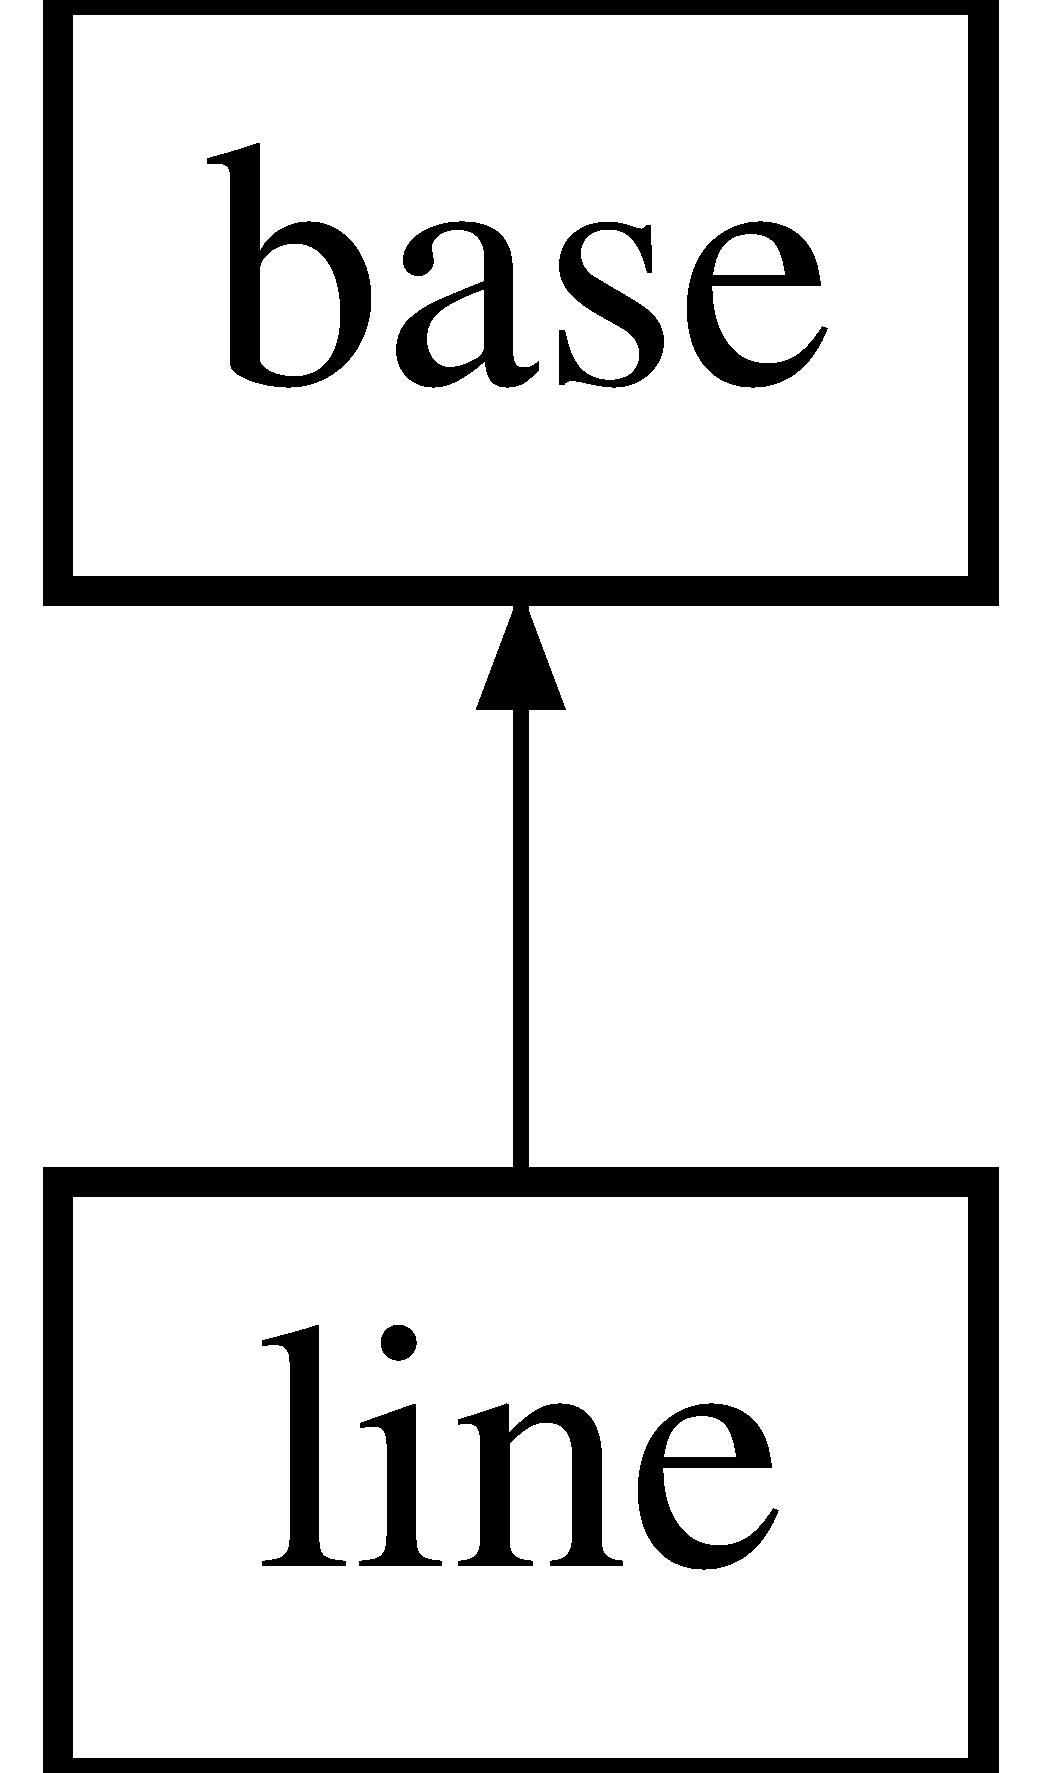
\includegraphics[height=2.000000cm]{classline}
\end{center}
\end{figure}
\subsection*{Public Member Functions}
\begin{DoxyCompactItemize}
\item 
\hypertarget{classline_a854d4e37d6dc6af1c7cd08cb801c6c26}{\hyperlink{classline_a854d4e37d6dc6af1c7cd08cb801c6c26}{line} ()}\label{classline_a854d4e37d6dc6af1c7cd08cb801c6c26}

\begin{DoxyCompactList}\small\item\em Default constructor. \end{DoxyCompactList}\item 
\hyperlink{classline_a62c98477491c4da965315766ee662ec8}{line} (\hyperlink{classpoint}{point} \&, \hyperlink{classpoint}{point} \&, string, \hyperlink{classdxf}{dxf} \&)
\begin{DoxyCompactList}\small\item\em Parameterized constructor. \end{DoxyCompactList}\end{DoxyCompactItemize}
\subsection*{Additional Inherited Members}


\subsection{Detailed Description}
Line entity class. 

Definition at line 172 of file dxf\-\_\-2\-D.\-h.



\subsection{Constructor \& Destructor Documentation}
\hypertarget{classline_a62c98477491c4da965315766ee662ec8}{\index{line@{line}!line@{line}}
\index{line@{line}!line@{line}}
\subsubsection[{line}]{\setlength{\rightskip}{0pt plus 5cm}line\-::line (
\begin{DoxyParamCaption}
\item[{{\bf point} \&}]{pt1, }
\item[{{\bf point} \&}]{pt2, }
\item[{string}]{dlayer, }
\item[{{\bf dxf} \&}]{d}
\end{DoxyParamCaption}
)}}\label{classline_a62c98477491c4da965315766ee662ec8}


Parameterized constructor. 

Initializes starting and ending points of line, specify the layer and calls write\-\_\-\-Line(x\-Start, y\-Start, z\-Start, x\-End, y\-End, z\-End, layer) function of dxf class for writing line entity to D\-X\-F file. 

Definition at line 43 of file dxf\-\_\-line.\-cpp.



The documentation for this class was generated from the following files\-:\begin{DoxyCompactItemize}
\item 
include/\hyperlink{dxf__2D_8h}{dxf\-\_\-2\-D.\-h}\item 
src/\hyperlink{dxf__line_8cpp}{dxf\-\_\-line.\-cpp}\end{DoxyCompactItemize}

\hypertarget{classpoint}{\section{point Class Reference}
\label{classpoint}\index{point@{point}}
}


Point entity class.  




{\ttfamily \#include $<$dxf\-\_\-2\-D.\-h$>$}

\subsection*{Public Member Functions}
\begin{DoxyCompactItemize}
\item 
\hyperlink{classpoint_a5fe21d4a4539320bf0f5caf1218d31c8}{point} ()
\begin{DoxyCompactList}\small\item\em Default constructor. \end{DoxyCompactList}\item 
\hypertarget{classpoint_add30ab9b6541ecd9322b989ff15f7cd3}{\hyperlink{classpoint_add30ab9b6541ecd9322b989ff15f7cd3}{point} (double, double y, double z=0)}\label{classpoint_add30ab9b6541ecd9322b989ff15f7cd3}

\begin{DoxyCompactList}\small\item\em Parameterised constructor. Default value of z is set to 0. \end{DoxyCompactList}\end{DoxyCompactItemize}
\subsection*{Public Attributes}
\begin{DoxyCompactItemize}
\item 
double \hyperlink{classpoint_aec4b8ad23ee8298cbf137c25906863cf}{x\-Co}
\item 
double \hyperlink{classpoint_a94a7f69d2ac81f8a229263aa743a0e6f}{y\-Co}
\item 
double \hyperlink{classpoint_a7a939155420b87e651d18dd364e017b1}{z\-Co}
\end{DoxyCompactItemize}


\subsection{Detailed Description}
Point entity class. 

Definition at line 90 of file dxf\-\_\-2\-D.\-h.



\subsection{Constructor \& Destructor Documentation}
\hypertarget{classpoint_a5fe21d4a4539320bf0f5caf1218d31c8}{\index{point@{point}!point@{point}}
\index{point@{point}!point@{point}}
\subsubsection[{point}]{\setlength{\rightskip}{0pt plus 5cm}point\-::point (
\begin{DoxyParamCaption}
{}
\end{DoxyParamCaption}
)}}\label{classpoint_a5fe21d4a4539320bf0f5caf1218d31c8}


Default constructor. 

Initializes x\-Co, y\-Co, z\-Co coordintes of point. 

Definition at line 29 of file dxf\-\_\-point.\-cpp.



\subsection{Member Data Documentation}
\hypertarget{classpoint_aec4b8ad23ee8298cbf137c25906863cf}{\index{point@{point}!x\-Co@{x\-Co}}
\index{x\-Co@{x\-Co}!point@{point}}
\subsubsection[{x\-Co}]{\setlength{\rightskip}{0pt plus 5cm}double point\-::x\-Co}}\label{classpoint_aec4b8ad23ee8298cbf137c25906863cf}
x-\/coordinate of point(x, y, z) 

Definition at line 94 of file dxf\-\_\-2\-D.\-h.

\hypertarget{classpoint_a94a7f69d2ac81f8a229263aa743a0e6f}{\index{point@{point}!y\-Co@{y\-Co}}
\index{y\-Co@{y\-Co}!point@{point}}
\subsubsection[{y\-Co}]{\setlength{\rightskip}{0pt plus 5cm}double point\-::y\-Co}}\label{classpoint_a94a7f69d2ac81f8a229263aa743a0e6f}
y-\/coordinate of point(x, y, z) 

Definition at line 94 of file dxf\-\_\-2\-D.\-h.

\hypertarget{classpoint_a7a939155420b87e651d18dd364e017b1}{\index{point@{point}!z\-Co@{z\-Co}}
\index{z\-Co@{z\-Co}!point@{point}}
\subsubsection[{z\-Co}]{\setlength{\rightskip}{0pt plus 5cm}double point\-::z\-Co}}\label{classpoint_a7a939155420b87e651d18dd364e017b1}
z-\/coordinate of point(x, y, z) 

Definition at line 94 of file dxf\-\_\-2\-D.\-h.



The documentation for this class was generated from the following files\-:\begin{DoxyCompactItemize}
\item 
include/\hyperlink{dxf__2D_8h}{dxf\-\_\-2\-D.\-h}\item 
src/\hyperlink{dxf__point_8cpp}{dxf\-\_\-point.\-cpp}\end{DoxyCompactItemize}

\hypertarget{classrectangle}{\section{rectangle Class Reference}
\label{classrectangle}\index{rectangle@{rectangle}}
}


Rectangle entity class.  




{\ttfamily \#include $<$dxf\-\_\-2\-D.\-h$>$}

Inheritance diagram for rectangle\-:\begin{figure}[H]
\begin{center}
\leavevmode
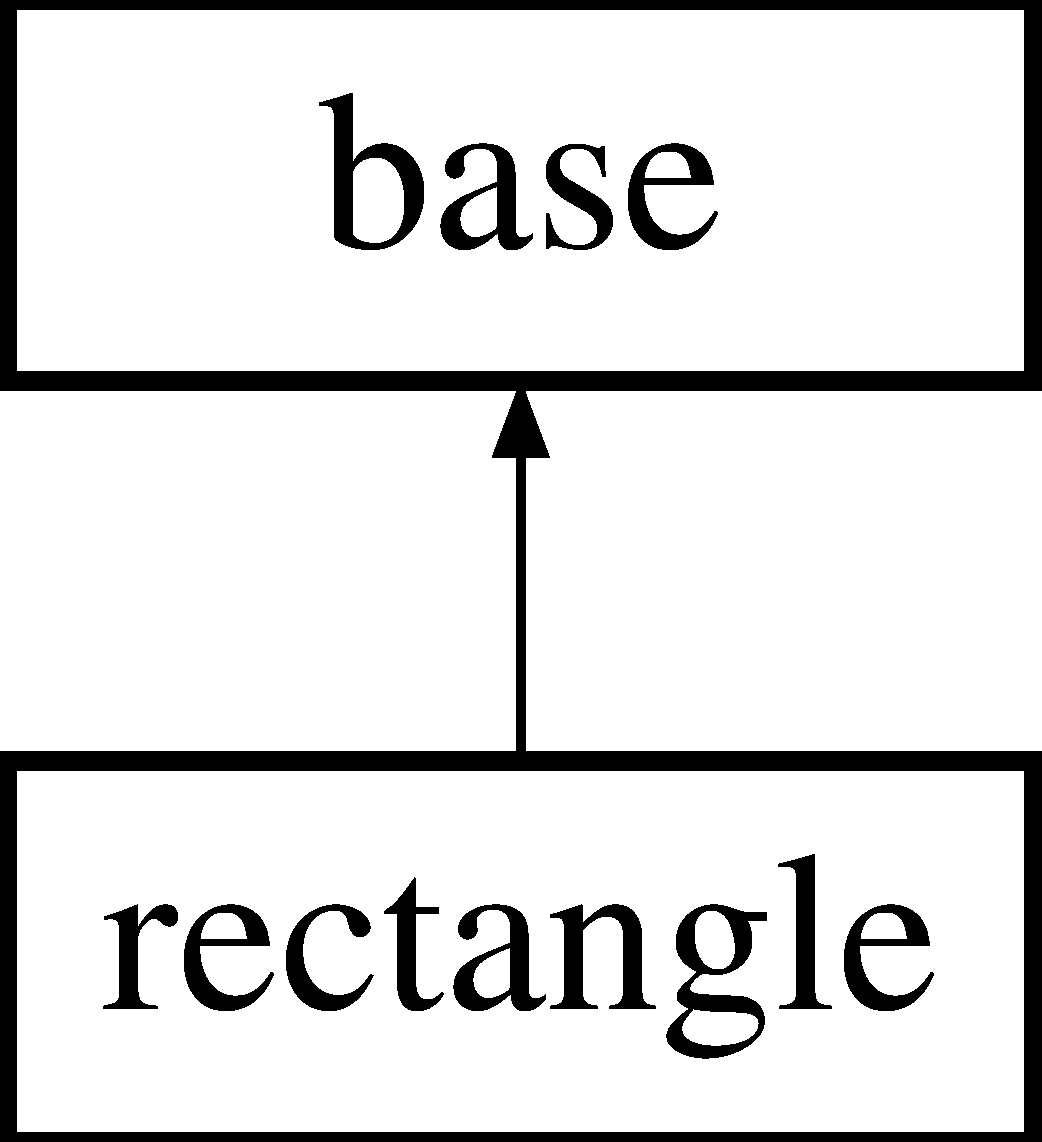
\includegraphics[height=2.000000cm]{classrectangle}
\end{center}
\end{figure}
\subsection*{Public Member Functions}
\begin{DoxyCompactItemize}
\item 
\hypertarget{classrectangle_acdc53c26d992570f77862a76aa6c07e7}{\hyperlink{classrectangle_acdc53c26d992570f77862a76aa6c07e7}{rectangle} ()}\label{classrectangle_acdc53c26d992570f77862a76aa6c07e7}

\begin{DoxyCompactList}\small\item\em Default constructor. \end{DoxyCompactList}\item 
\hyperlink{classrectangle_a2b6c06e9b26e4b69a3219f7d68040cf0}{rectangle} (\hyperlink{classpoint}{point} \&, \hyperlink{classpoint}{point} \&, string, \hyperlink{classdxf}{dxf} \&)
\begin{DoxyCompactList}\small\item\em Parameterized constructor. \end{DoxyCompactList}\item 
\hyperlink{classrectangle_ad057163264d95fa833a1ad9887a78d0c}{rectangle} (\hyperlink{classpoint}{point} \&, \hyperlink{classpoint}{point} \&, string, \hyperlink{classdxf}{dxf} \&, int hflag, int hcolor=256)
\begin{DoxyCompactList}\small\item\em Parameterized constructor for solid fill. \end{DoxyCompactList}\item 
\hypertarget{classrectangle_af6b2a94031985fe184fc0b7bb5466822}{\hyperlink{classrectangle_af6b2a94031985fe184fc0b7bb5466822}{rectangle} (\hyperlink{classpoint}{point} \&, \hyperlink{classpoint}{point} \&, string, \hyperlink{classdxf}{dxf} \&, int hflag, string p\-\_\-name, int hcolor=256)}\label{classrectangle_af6b2a94031985fe184fc0b7bb5466822}

\begin{DoxyCompactList}\small\item\em Parameterized constructor. \end{DoxyCompactList}\end{DoxyCompactItemize}
\subsection*{Additional Inherited Members}


\subsection{Detailed Description}
Rectangle entity class. 

Definition at line 219 of file dxf\-\_\-2\-D.\-h.



\subsection{Constructor \& Destructor Documentation}
\hypertarget{classrectangle_a2b6c06e9b26e4b69a3219f7d68040cf0}{\index{rectangle@{rectangle}!rectangle@{rectangle}}
\index{rectangle@{rectangle}!rectangle@{rectangle}}
\subsubsection[{rectangle}]{\setlength{\rightskip}{0pt plus 5cm}rectangle\-::rectangle (
\begin{DoxyParamCaption}
\item[{{\bf point} \&}]{pt1, }
\item[{{\bf point} \&}]{pt2, }
\item[{string}]{dlayer, }
\item[{{\bf dxf} \&}]{d}
\end{DoxyParamCaption}
)}}\label{classrectangle_a2b6c06e9b26e4b69a3219f7d68040cf0}


Parameterized constructor. 

Initializes starting and ending points of rectangle, specify the layer and calls write\-\_\-\-Rect(x\-Start, y\-Start, z\-Start, x\-End, y\-End, z\-End, layer) function of dxf class for writing rectangle entity to D\-X\-F file. 

Definition at line 44 of file dxf\-\_\-rect.\-cpp.

\hypertarget{classrectangle_ad057163264d95fa833a1ad9887a78d0c}{\index{rectangle@{rectangle}!rectangle@{rectangle}}
\index{rectangle@{rectangle}!rectangle@{rectangle}}
\subsubsection[{rectangle}]{\setlength{\rightskip}{0pt plus 5cm}rectangle\-::rectangle (
\begin{DoxyParamCaption}
\item[{{\bf point} \&}]{pt1, }
\item[{{\bf point} \&}]{pt2, }
\item[{string}]{dlayer, }
\item[{{\bf dxf} \&}]{d, }
\item[{int}]{hflag, }
\item[{int}]{hcolor = {\ttfamily 256}}
\end{DoxyParamCaption}
)}}\label{classrectangle_ad057163264d95fa833a1ad9887a78d0c}


Parameterized constructor for solid fill. 

Initialize starting and ending points of rectangle, specify the layer, flag = 1 for solid fill and calls write\-\_\-\-Rect(x\-Start, y\-Start, z\-Start, x\-End, y\-End, z\-End, layer, flag, color) function of dxf class for writing rectangle (solid fill) entity to D\-X\-F file. 

Definition at line 76 of file dxf\-\_\-rect.\-cpp.



The documentation for this class was generated from the following files\-:\begin{DoxyCompactItemize}
\item 
include/\hyperlink{dxf__2D_8h}{dxf\-\_\-2\-D.\-h}\item 
src/\hyperlink{dxf__rect_8cpp}{dxf\-\_\-rect.\-cpp}\end{DoxyCompactItemize}

\chapter{File Documentation}
\hypertarget{dxf__2D_8h}{\section{include/dxf\-\_\-2\-D.h File Reference}
\label{dxf__2D_8h}\index{include/dxf\-\_\-2\-D.\-h@{include/dxf\-\_\-2\-D.\-h}}
}
{\ttfamily \#include $<$cmath$>$}\\*
{\ttfamily \#include $<$cstring$>$}\\*
{\ttfamily \#include $<$fstream$>$}\\*
{\ttfamily \#include $<$iostream$>$}\\*
\subsection*{Classes}
\begin{DoxyCompactItemize}
\item 
class \hyperlink{classbase}{base}
\begin{DoxyCompactList}\small\item\em Base class defines functions for D\-X\-F header, footer and hatching section. \end{DoxyCompactList}\item 
class \hyperlink{classpoint}{point}
\begin{DoxyCompactList}\small\item\em Point entity class. \end{DoxyCompactList}\item 
class \hyperlink{classdxf}{dxf}
\begin{DoxyCompactList}\small\item\em Draw entities in D\-X\-F file. \end{DoxyCompactList}\item 
class \hyperlink{classline}{line}
\begin{DoxyCompactList}\small\item\em Line entity class. \end{DoxyCompactList}\item 
class \hyperlink{classcircle}{circle}
\begin{DoxyCompactList}\small\item\em Circle entity class. \end{DoxyCompactList}\item 
class \hyperlink{classrectangle}{rectangle}
\begin{DoxyCompactList}\small\item\em Rectangle entity class. \end{DoxyCompactList}\end{DoxyCompactItemize}


\subsection{Detailed Description}
This is a header file that declare classes for creating 2\-D drawings.

\begin{DoxyVersion}{Version}
0.\-1 
\end{DoxyVersion}
\begin{DoxyDate}{Date}
03/19/2013 01\-:34\-:03 P\-M Compiler gcc
\end{DoxyDate}
\begin{DoxyAuthor}{Author}
Avneet Kaur, \href{mailto:kauravneet958@gmail.com}{\tt kauravneet958@gmail.\-com} License G\-N\-U General Public License 
\end{DoxyAuthor}
\begin{DoxyCopyright}{Copyright}
Copyright (c) 2013, Great\-Developers \href{https://github.com/GreatDevelopers}{\tt https\-://github.\-com/\-Great\-Developers} 
\end{DoxyCopyright}


Definition in file \hyperlink{dxf__2D_8h_source}{dxf\-\_\-2\-D.\-h}.


\hypertarget{dxf__base_8cpp}{\section{src/dxf\-\_\-base.cpp File Reference}
\label{dxf__base_8cpp}\index{src/dxf\-\_\-base.\-cpp@{src/dxf\-\_\-base.\-cpp}}
}


This file defines base class. base class is used to write header, footer and common hatching part to D\-X\-F file.  


{\ttfamily \#include \char`\"{}../include/dxf\-\_\-2\-D.\-h\char`\"{}}\\*


\subsection{Detailed Description}
This file defines base class. base class is used to write header, footer and common hatching part to D\-X\-F file. \begin{DoxyVersion}{Version}
0.\-1 
\end{DoxyVersion}
\begin{DoxyDate}{Date}
03/19/2013 09\-:30\-:23 P\-M Compiler gcc
\end{DoxyDate}
\begin{DoxyAuthor}{Author}
Avneet Kaur, \href{mailto:kauravneet958@gmail.com}{\tt kauravneet958@gmail.\-com} License G\-N\-U General Public License 
\end{DoxyAuthor}
\begin{DoxyCopyright}{Copyright}
Copyright (c) 2013, Great\-Developers \href{https://github.com/GreatDevelopers}{\tt https\-://github.\-com/\-Great\-Developers} 
\end{DoxyCopyright}


Definition in file \hyperlink{dxf__base_8cpp_source}{dxf\-\_\-base.\-cpp}.


\hypertarget{dxf__circle_8cpp}{\section{src/dxf\-\_\-circle.cpp File Reference}
\label{dxf__circle_8cpp}\index{src/dxf\-\_\-circle.\-cpp@{src/dxf\-\_\-circle.\-cpp}}
}


This file defines circle class. circle class is used to create circle entity with or without hatching.  


{\ttfamily \#include \char`\"{}../include/dxf\-\_\-2\-D.\-h\char`\"{}}\\*


\subsection{Detailed Description}
This file defines circle class. circle class is used to create circle entity with or without hatching. \begin{DoxyVersion}{Version}
0.\-1 
\end{DoxyVersion}
\begin{DoxyDate}{Date}
03/19/2013 09\-:30\-:23 P\-M Compiler gcc
\end{DoxyDate}
\begin{DoxyAuthor}{Author}
Avneet Kaur, \href{mailto:kauravneet958@gmail.com}{\tt kauravneet958@gmail.\-com} License G\-N\-U General Public License 
\end{DoxyAuthor}
\begin{DoxyCopyright}{Copyright}
Copyright (c) 2013, Great\-Developers \href{https://github.com/GreatDevelopers}{\tt https\-://github.\-com/\-Great\-Developers} 
\end{DoxyCopyright}


Definition in file \hyperlink{dxf__circle_8cpp_source}{dxf\-\_\-circle.\-cpp}.


\hypertarget{dxf__dxf_8cpp}{\section{src/dxf\-\_\-dxf.cpp File Reference}
\label{dxf__dxf_8cpp}\index{src/dxf\-\_\-dxf.\-cpp@{src/dxf\-\_\-dxf.\-cpp}}
}


This file defines dxf class. dxf class is used to draw multiple entites in a D\-X\-F file.  


{\ttfamily \#include \char`\"{}../include/dxf\-\_\-2\-D.\-h\char`\"{}}\\*


\subsection{Detailed Description}
This file defines dxf class. dxf class is used to draw multiple entites in a D\-X\-F file. \begin{DoxyVersion}{Version}
0.\-1 
\end{DoxyVersion}
\begin{DoxyDate}{Date}
03/19/2013 09\-:10\-:35 P\-M Compiler gcc
\end{DoxyDate}
\begin{DoxyAuthor}{Author}
Avneet Kaur, \href{mailto:kauravneet958@gmail.com}{\tt kauravneet958@gmail.\-com} License G\-N\-U General Public License 
\end{DoxyAuthor}
\begin{DoxyCopyright}{Copyright}
Copyright (c) 2013, Great\-Developers \href{https://github.com/GreatDevelopers}{\tt https\-://github.\-com/\-Great\-Developers} 
\end{DoxyCopyright}


Definition in file \hyperlink{dxf__dxf_8cpp_source}{dxf\-\_\-dxf.\-cpp}.


\hypertarget{dxf__line_8cpp}{\section{src/dxf\-\_\-line.cpp File Reference}
\label{dxf__line_8cpp}\index{src/dxf\-\_\-line.\-cpp@{src/dxf\-\_\-line.\-cpp}}
}


This file is defining line class. line class is used to create line entity.  


{\ttfamily \#include \char`\"{}../include/dxf\-\_\-2\-D.\-h\char`\"{}}\\*


\subsection{Detailed Description}
This file is defining line class. line class is used to create line entity. \begin{DoxyVersion}{Version}
0.\-1 
\end{DoxyVersion}
\begin{DoxyDate}{Date}
03/19/2013 09\-:10\-:35 P\-M Compiler gcc
\end{DoxyDate}
\begin{DoxyAuthor}{Author}
Avneet Kaur, \href{mailto:kauravneet958@gmail.com}{\tt kauravneet958@gmail.\-com} License G\-N\-U General Public License 
\end{DoxyAuthor}
\begin{DoxyCopyright}{Copyright}
Copyright (c) 2013, Great\-Developers \href{https://github.com/GreatDevelopers}{\tt https\-://github.\-com/\-Great\-Developers} 
\end{DoxyCopyright}


Definition in file \hyperlink{dxf__line_8cpp_source}{dxf\-\_\-line.\-cpp}.


\hypertarget{dxf__point_8cpp}{\section{src/dxf\-\_\-point.cpp File Reference}
\label{dxf__point_8cpp}\index{src/dxf\-\_\-point.\-cpp@{src/dxf\-\_\-point.\-cpp}}
}


This file defines point class. point class is used to initialize x\-Co, y\-Co and z\-Co coordinates of point.  


{\ttfamily \#include \char`\"{}../include/dxf\-\_\-2\-D.\-h\char`\"{}}\\*


\subsection{Detailed Description}
This file defines point class. point class is used to initialize x\-Co, y\-Co and z\-Co coordinates of point. \begin{DoxyVersion}{Version}
0.\-1 
\end{DoxyVersion}
\begin{DoxyDate}{Date}
03/19/2013 09\-:30\-:23 P\-M Compiler gcc
\end{DoxyDate}
\begin{DoxyAuthor}{Author}
Avneet Kaur, \href{mailto:kauravneet958@gmail.com}{\tt kauravneet958@gmail.\-com} License G\-N\-U General Public License 
\end{DoxyAuthor}
\begin{DoxyCopyright}{Copyright}
Copyright (c) 2013, Great\-Developers \href{https://github.com/GreatDevelopers}{\tt https\-://github.\-com/\-Great\-Developers} 
\end{DoxyCopyright}


Definition in file \hyperlink{dxf__point_8cpp_source}{dxf\-\_\-point.\-cpp}.


\hypertarget{dxf__rect_8cpp}{\section{src/dxf\-\_\-rect.cpp File Reference}
\label{dxf__rect_8cpp}\index{src/dxf\-\_\-rect.\-cpp@{src/dxf\-\_\-rect.\-cpp}}
}


This file defines rectangle class. rectangle class is used to create rectangle with or without hatching.  


{\ttfamily \#include \char`\"{}../include/dxf\-\_\-2\-D.\-h\char`\"{}}\\*


\subsection{Detailed Description}
This file defines rectangle class. rectangle class is used to create rectangle with or without hatching. \begin{DoxyVersion}{Version}
0.\-1 
\end{DoxyVersion}
\begin{DoxyDate}{Date}
03/19/2013 09\-:30\-:23 P\-M Compiler gcc
\end{DoxyDate}
\begin{DoxyAuthor}{Author}
Avneet Kaur, \href{mailto:kauravneet958@gmail.com}{\tt kauravneet958@gmail.\-com} License G\-N\-U General Public License 
\end{DoxyAuthor}
\begin{DoxyCopyright}{Copyright}
Copyright (c) 2013, Great\-Developers \href{https://github.com/GreatDevelopers}{\tt https\-://github.\-com/\-Great\-Developers} 
\end{DoxyCopyright}


Definition in file \hyperlink{dxf__rect_8cpp_source}{dxf\-\_\-rect.\-cpp}.


\addcontentsline{toc}{part}{Index}
\printindex
\end{document}
